\documentclass[a4paper,11pt]{article}
\usepackage[utf8]{inputenc}
\usepackage{amsmath}
\usepackage{amsfonts}
\usepackage{amssymb}
\usepackage{graphicx}
\usepackage{braket}

\numberwithin{equation}{section}
\renewcommand\thesubsection{\alph{subsection}}
\newcommand{\bvp}[1]{\mathbf{#1}'}
\newcommand{\bv}[1]{\mathbf{#1}}
\newcommand{\ez}{\epsilon_0}
\newcommand{\eo}{\epsilon_1}
\newcommand{\lrp}[1]{\left({#1}\right)}
\newcommand{\lrb}[1]{\left\{{#1}\right\}}


%opening
\title{Electromagnetic Theory HW6}
\author{Vince Baker}

\begin{document}

\maketitle

\section{3.9}
The conventional solution in cylindrical coordinates takes the seperation constant $k^2$, resulting in $\sinh, \cosh$ solutions for the z equation.
In this problem we have boundary conditions $\Phi(\rho,\phi,0)=0$ and $\Phi(\rho,\phi,L)=0$.
These cannot be satisfied by the hyperbolic functions.
Instead, we take the separation constant to be $-k^2$ so that we get the $\sin$ solution for z which will satisfy the boundary conditions.
We are then working with the modified Bessel functions.\\
We are looking for an interior solution, so we discard the Neumann terms. 
The $\phi$ solutions are the typical exponential combinations, with the usual integer restriction on $m$ so they are single-valued.
We can then write the general solution in cylindrical coordinates:
\begin{align}
 \Phi(\rho,\phi,z) &= \sum_{m=0}^\infty \sum_{n=1}^\infty I_m(\frac{n\pi}{L}\rho)\sin{\lrp{\frac{n\pi}{L}z}}\lrp{A_{mn}e^{im\phi}+B_{mn}e^{-im\phi}}
\end{align}
Where we have removed the $n=0$ term, since it will be zero due to the sine function.\\
We now solve for the coefficients using the other provided boundary condition:
\begin{align}
 \Phi(b,\phi,z) &= V(\phi,z)\\
 V(\phi,z) &= \sum_{m=0}^\infty \sum_{n=1}^\infty I_m(\frac{n\pi}{L}b)\sin{\lrp{\frac{n\pi}{L}z}}\lrp{A_{mn}e^{im\phi}+B_{mn}e^{-im\phi}}
\end{align}
We multiply both sides by a $e^{-im'\phi}\sin{\frac{n\pi}{L}z'}$ and integrate, using the delta function relations:
\begin{align}
 \int_0^{2\pi} e^{i(m-m')\phi}\ d\phi &= 2\pi\delta(m-m')\\
 \int_0^L \sin(n\pi z/L)\sin(n'\pi z/L)\ dz &= \frac{L}{2}\delta(n-n')
\end{align}
We then have:
\begin{gather}
 \int_0^{2\pi} \int_0^L V(\phi,z)e^{-im\phi}\sin{\lrp{\frac{n\pi}{L}z}}\ d\phi\ dz =  I_m(\frac{n\pi}{L}b) \pi L A_{mn}\\
 A_{mn} = \lrp{I_m(\frac{n\pi}{L}b) \pi L}^{-1} \int_0^{2\pi} \int_0^L V(\phi,z)e^{-im\phi}\sin{\lrp{\frac{n\pi}{L}z}}\ d\phi\ dz
\end{gather}
Following the same process, but multiplying by $e^{im'\phi}\sin{\lrp{\frac{n\pi}{L}z'}}$, we find the $B_{mn}$:
\begin{gather}
 B_{mn} = \lrp{I_m(\frac{n\pi}{L}b) \pi L}^{-1} \int_0^{2\pi} \int_0^L V(\phi,z)e^{im\phi}\sin{\lrp{\frac{n\pi}{L}z}}\ d\phi\ dz
\end{gather}
Inserting the coefficients into (1) we now have a complete expression for the potential inside the cylinder.


\section{4.1}
a) The charge distribution consists of 4 point charges, all at $r=a$ and $\theta = \pi/2$.
The four $\phi$ angles are $0, \pm\pi/2, \pi$. 
We can write the charge distribution in terms of delta functions:
\begin{align}
 \rho &= q\delta(r-a)\delta(\theta-\pi/2)\lrb{\delta(\phi)+\delta(\phi-\pi/2)-\delta(\phi-\pi/2)-\delta(\phi-\pi)}
\end{align}
The coefficients are then:
\begin{align}
 q_{\ell m} &= \int Y_{\ell m}^*(\theta,\phi)r^\ell \rho(\bv{x}) d^3x\\
 q_{\ell m} &= qa^\ell \lrp{Y_{\ell m}^*(0,0)+Y_{\ell m}^*(0,\pi/2)-Y_{\ell m}^*(0,-\pi/2)-Y_{\ell m}^*(0,\pi)}
\end{align}
We pull out the common $\theta$ part of the spherical harmonics:
\begin{align}
 q_{\ell m} &= qa^\ell P_\ell(0)\sqrt{ \frac{(2\ell+1)(\ell-m)!}{4\pi(\ell+m)!} } \lrp{e^{im0}+e^{im\pi/2}-e^{-im\pi/2}-e^{im\pi}}
\end{align}
When m is even the first and last $\phi$ terms will cancel, as will the second and third. Therefore $q_{\ell m}=0$ for m even.
When m is odd the $\phi$ terms reduce to $2\mp2i$ with the sign alternating.
We can then write the coefficients as:
\begin{align}
 q_{\ell m} &= 2qa^\ell P_\ell(0)\sqrt{ \frac{(2\ell+1)(\ell-m)!}{4\pi(\ell+m)!} } \lrp{1-i^m}\ (\text{m odd})
\end{align}
\\
b) The charge density in b consists of three point charges, so we again write the charge density in terms of delta functions:
\begin{align}
 \rho &= -\frac{2q}{4\pi}(\delta(r))+\frac{q}{2\pi a^2}\delta(r-a)\lrp{\delta(\theta)+\delta(\theta-\pi)}
\end{align}
We note that, since there are no delta functions in $\phi$, the $\phi$ integral will be:
\begin{align}
 \int_0^{2\pi}e^{im\phi}d\phi &= 0\ (\phi\ne 0)\\
      &= 2\pi\ (\phi=0)
\end{align}
Doing the integral for the first term in (6) we separate the spherical harmonic term into $\phi$ and $\theta$.
With $m=0$ the $\theta$ part is just the normal Legendre function.
Since the integral $\int_0^\pi P_\ell(\cos\theta)\sin{\theta}\ d\theta$ is zero for $\ell\ne 0$ we have a single term at $\ell=0,m=0$.
\begin{align}
 q^1_{0,0} &= -\frac{q}{\sqrt{\pi}}
\end{align}
We now address the second term in (6).
\begin{align}
\begin{split}
 q^2_{\ell,0} = &\frac{q}{a^2} \sqrt{\frac{2\ell+1}{4\pi}}\int_0^\pi r^{\ell+2} \delta(r-a) \ dr \\
		&\times \int_0^\infty P_\ell(\cos{\theta})\sin{\theta} \lrb{\delta(\theta)+\delta(\theta-\pi)}\ d\theta
\end{split}\\
 q^2_{\ell,0} &= qa^\ell\sqrt{\frac{2\ell+1}{4\pi}} \int_0^\pi  P_\ell(\cos{\theta})\sin{\theta} \lrb{\delta(\theta)+\delta(\theta-\pi)}\ d\theta\\
 q^2_{\ell,0} &= qa^\ell\sqrt{\frac{2\ell+1}{4\pi}} \lrb{P_\ell(1)-P_\ell(-1)}\\
 q^2_{\ell,0} &= 2qa^\ell\sqrt{\frac{2\ell+1}{4\pi}}\ (\ell=0,2,4...)
\end{align}
So we have:
\begin{align}
 q_{0,0} &= -\frac{q}{\sqrt{\pi}}+2q\sqrt{\frac{1}{4\pi}}=0\\
 q_{\ell,0} &= 0\ (\ell \text{ odd})\\
 q_{\ell,0} &= 2qa^\ell\sqrt{\frac{2\ell+1}{4\pi}}\ (\ell \text{ even})
\end{align}
\\
c) The expansion of the potential in spherical harmonics has the form:
\begin{align}
 \Phi(\bv{x}) &= \frac{1}{4\pi\ez}\sum_{\ell=0}^\infty \sum_{m=-\ell}^\ell \frac{4\pi}{2\ell+1}q_{\ell,m}\frac{Y_{\ell m}(\theta,\phi)}{r^{\ell+1}}
\end{align}
The lowest order nonzero term is $\ell=2,m=0$.
Using the $q_{\ell,m}$ found above:
\begin{align}
 \Phi(\bv{x}) &\simeq \frac{1}{4\pi\ez}\sqrt{\frac{4\pi}{5}}\lrb{2qa^2\sqrt{\frac{5}{4\pi}}}\frac{Y_{2,0}(\theta,\phi)}{r^3}\\
 \Phi(\bv{x}) &\simeq \frac{q}{4\pi\ez}\frac{a^2}{r^3}\lrp{3\cos^2{(\theta})-1}
\end{align}
In this x-y plane, with azimuthal symmetry, the potential is:
\begin{align}
 \Phi(r) &\simeq -\frac{q}{4\pi\ez}\frac{a^2}{r^3}
\end{align}
d) Caclulating the potential directly from Coulomb's law in the x-y plane we have:
\begin{align}
 \Phi(r) &= \frac{1}{4\pi\ez}\lrb{\frac{-2q}{r}+\frac{q}{\sqrt{r^2+a^2}}+\frac{q}{\sqrt{r^2+a^2}} }\\
 \Phi(r) &= \frac{q}{4\pi\ez}\lrb{\frac{2}{\sqrt{r^2+a^2}}-\frac{2}{r}}\\
\end{align}
We now plot both our approximation using the lowest-order term in the spehrical harmonic expansion and the exact result.
We choose length dimensions in a and our constants such that $\frac{q}{4\pi\ez}=1$. 
The lowest-term approximation is quite good for distances farther than one or two $a$, but breaks down very close to the charges.\\
\\
\begin{figure}[h]
 \caption{Approximate and exact potentials on x-y plane}
 \centering
   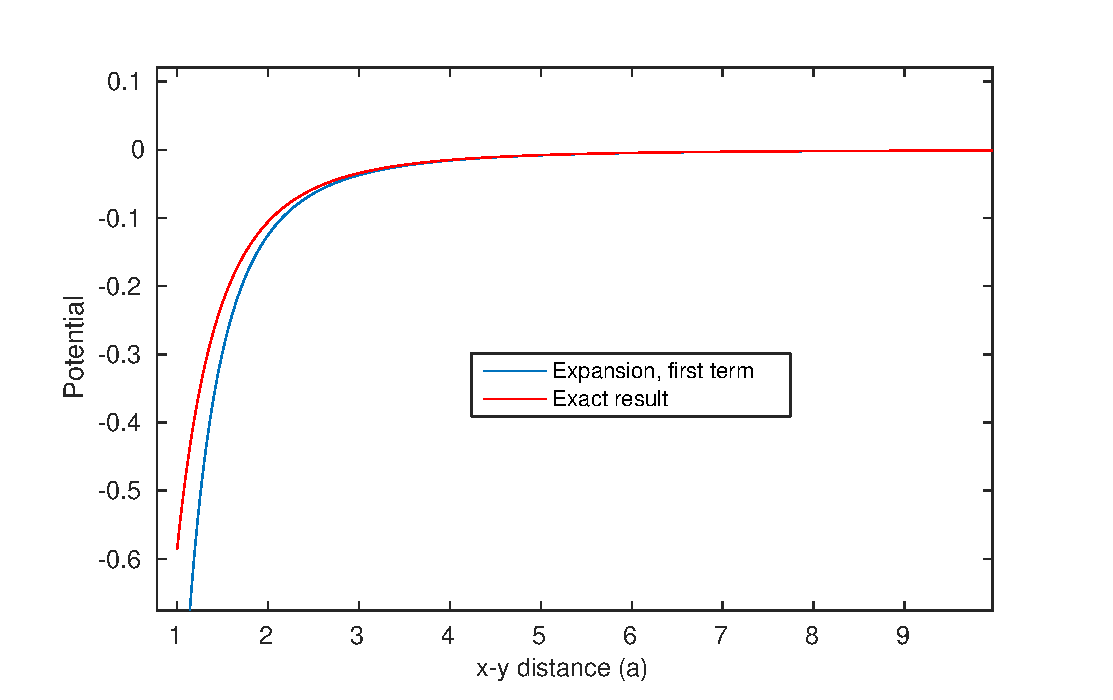
\includegraphics[width=\textwidth]{p41}
\end{figure}

\section{4.9}
a) We solve the problem using the method of images with the appropriate boundary conditions at the surface of the dielectric sphere:
\begin{align}
 (\bv{D}_2-\bv{D}_1)\cdot \hat{n} &= 0\ \text{(no surface charge)}\\
 \bv{E}_2 \times \bv{E}_1 &= 0
\end{align}
Following a similar approach to the planar method of images, we'll place an image charge $q'$ inside the sphere at $a^2/d$.
We will also place a second image charge $q''$ at the location of the actual charge.
The second image charge will allow us to solve for the potential inside the sphere.\\
The problem is simpler if we place the center of the sphere at the origin and place the charge on the z axis.
With azimuthal symmetry the harmonic expansion terms with $m\ne 0$ will be zero, and we will work with the regular Legendre functions.
The general expansion of the inverse distance is then:
\begin{align}
 \frac{1}{|\bv{x}-\bvp{x}|} &= \sum_{\ell=0}^\infty \frac{r_<^\ell}{r_>^{\ell+1}}P_\ell (\cos\theta)
\end{align}
We'll end up with expressions for three regions: $r<a,a<r<d,r>d$.
We examine the first two, since they will be used with the boundary conditions.
The expression for $a<r<d$ includes the potential due to both the actual charge and the image charge $q'$at $a^2/d$:
\begin{align}
 \Phi_{r>a} &= \frac{1}{4\pi\ez}\sum_{\ell=0}^\infty P_\ell(\cos\theta)\lrb{ \frac{qr^\ell}{d^{\ell+1}}+q'\lrp{\frac{a^2}{d}}^{\ell+1}\frac{1}{r^{\ell+1}} }
\end{align}
For the solution inside the sphere we are only interested in the region where $r>a^2/d$:
\begin{align}
 \Phi_{r<a} &= \frac{1}{4\pi\epsilon}\sum_{\ell=0}^\infty P_\ell(\cos\theta)q''\frac{1}{r^{\ell+1}}\frac{a^{2\ell}}{d^\ell}
\end{align}
We now apply the boundary conditions (1) and (2) to the potential inside (5) and outside (4) the surface of the dielectric sphere, with the sums equal term-by-term.
\begin{align}
 \ez\frac{\partial \Phi_{r>a}}{\partial r} &= \epsilon \frac{\partial \Phi_{r<a}}{\partial r}\\
 q\ell\frac{r^{\ell-1}}{d^{\ell+1}}-(\ell+1)q'\lrp{\frac{a^2}{d}}^\ell\frac{1}{r^\ell} &= lq'' \frac{r^{\ell-1}}{d^{\ell+1}}\\
 (q-q'') &= q' \frac{d^{\ell+1}}{r^{2\ell+1}}\lrp{\frac{a^2}{d}}^\ell\frac{\ell+1}{\ell}\\
 (q-q'') &= q' \frac{d}{a}\frac{\ell+1}{\ell}
\end{align}
Applying the tangential boundary condition:
\begin{align}
 \frac{\partial \Phi_{r>a}}{\partial \theta} &= \frac{\partial \Phi_{r<a}}{\partial \theta}\\
 \frac{1}{\ez}\lrp{q\frac{a^\ell}{d^{\ell+1}}}+q'\lrp{\frac{a^2}{d}}^\ell\frac{1}{a^{\ell+1}} &= \frac{1}{\epsilon}q''\frac{a^\ell}{d^{\ell+1}}\\
 \frac{\epsilon}{\ez}q-q'' &= -\frac{\epsilon}{\ez}\frac{d}{a}q'
\end{align}
We can then solve equations (9) and (12) to find:
\begin{align}
 q' &= \lrp{\frac{a}{d}\frac{\epsilon/\ez-1}{\epsilon/\ez-(\ell+1)/\ell}}q\\
 q'' &= \lrp{ \frac{1}{\frac{\ez}{\epsilon}(\ell+1)-\ell }}q
\end{align}
With the magnitude of the image charges determined the potential at every point in space is determined by combining the potentials of the relevant point charges.
\\
\\
b) Plugging in the value for $q''$ the potential close to the center of the sphere is:
\begin{align}
 \Phi_{r<a^2/d} &= \frac{q}{4\pi\epsilon} \sum_{\ell=0}^\infty \lrp{ \frac{1}{\frac{\ez}{\epsilon}(\ell+1)-\ell }} \frac{r^\ell}{d^{\ell+1}}P_\ell(\cos\theta)
\end{align}
As $r\rightarrow 0$ only the $\ell=0$ term survives:
\begin{align}
 \Phi_{\ell=0} &= \frac{q}{4\pi\ez d}
\end{align}
This doesn't have any dependence on the coordinates so the field would be zero. 
Since that's clearly not right, we keep another term in the sum:
\begin{align}
 \Phi_{\ell=1} &= \frac{1}{4\pi \epsilon}\frac{1}{2\ez/\epsilon-1}\frac{r}{d^2}\cos{(\theta)}
\end{align}
Recognizing that $r\cos{(\theta)}=z$ the gradient of this term gives us the electric field:
\begin{align}
 E &= -\nabla \Phi = -\frac{1}{4\pi\epsilon d^2}\frac{1}{2\ez/\epsilon-1} \hat{z}
\end{align}
This is the electric field strength for the point charge modified by a factor that includes the relative permittivity of the dielectric of the sphere.

\end{document}
